\documentclass{ximera}
\title{Results}
\outcome{Understand past evidence of Ximera's success}

\begin{document}
\begin{abstract}
  How Ximera performs verses commerical solutions.
\end{abstract}
\maketitle

Thousands of students have now used Ximera, and the platform has been
used at six institutions.  Compared to those using a commercial
textbook, students using Ximera do just as well on exams, and by some
affective measures, perhaps do better.


\paragraph{Equally well on exams}

\begin{center}
  \begin{tabular}{rrr}
    \hline
    & ABC & DFWI \\ 
    \hline
    closed-source & 1427 & 480 \\ 
    open-source & 108 &  37 \\ 
    \hline
  \end{tabular}
\end{center}
    
No significant difference in exam scores for students using the
closed-source textbook \textcolor{gray}{(\(M \approx 340\),
  \(SD \approx 93.1\))}.  and students using the open-source textbook
\textcolor{gray}{(\(M \approx 347\), \(SD \approx 73.1\));}
\textcolor{gray}{\(t( 119.91 ) = -0.86\), \(p\approx 0.39\).}

\paragraph{Affective improvements}

Students in the open-source section were more likely to express
post-course the same level or a stronger level of agreement with the
confidence item as pre-course \textcolor{gray}{\(OR = 1.42\), 95\% CI
  \([ 0.98 , 2.06 ]\), \(p\approx 0.071\).}

Students in the open-source section were more likely to express
post-course the same level or a stronger level of agreement with the
enjoyment item as pre-course \textcolor{gray}{\(OR = 1.43\), 95\% CI
  \([ 0.98 , 2.1 ]\), \(p\approx 0.072\).}

\paragraph{Readability}

Among students at large PhD granting instiutions, about 77.3\% agree
that their assigned textbook is readable.  At Ohio State, about 71.1\%
of participants in the commercial textbook sections agreed to the
readability items, as compared to 85\% of particpants in the
open-source sections.  The the participants using the open-source
textbook were more likely to agree the their textbook was readable as
compared to the participants using the closed-source text,
\(OR = 2.48\), 95\% CI \([ 1.53 , 4.28 ]\), \(p < 0.001\).

\begin{image}
  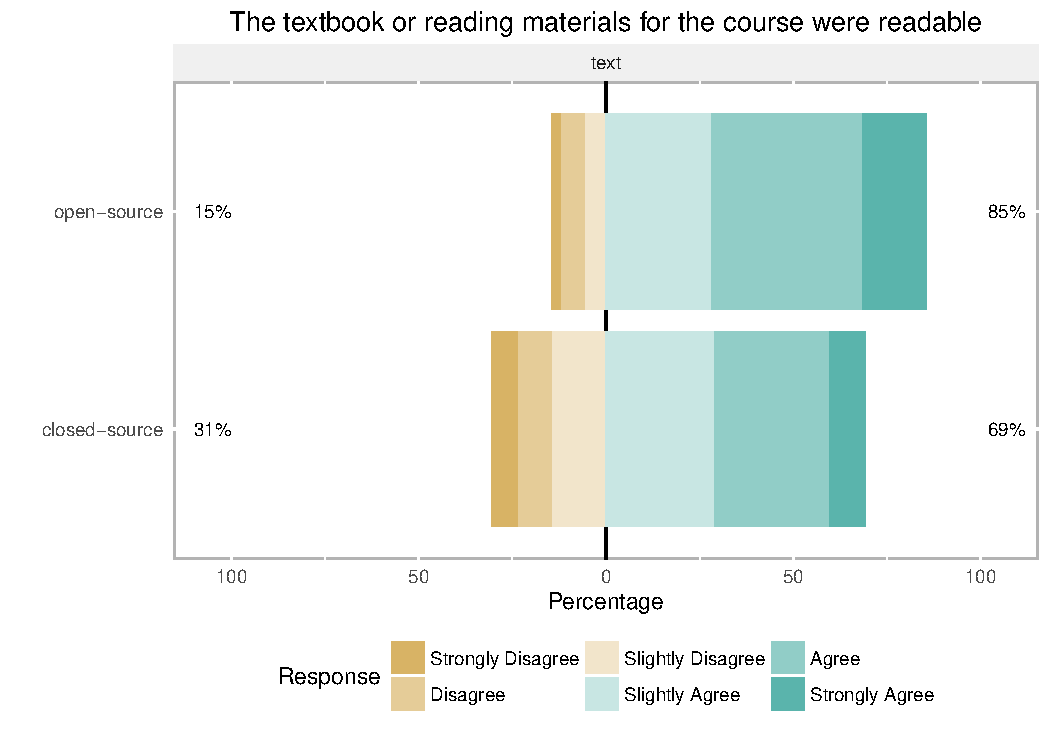
\includegraphics{more-readable.pdf}
\end{image}

Significant difference in exam scores for students who agreed that the
textbook was readable \textcolor{gray}{(\(M \approx 363\),
  \(SD \approx 70\))} compared to those who disagreed
\textcolor{gray}{(\(M \approx 344\), \(SD \approx 74.4\));}
\textcolor{gray}{\(t( 680.19 ) = -4.06\), \(p < 0.001\).}

\end{document}

%%% Local Variables:
%%% mode: latex
%%% TeX-master: t
%%% End:
